% Quelle der Abbildung "Datenfluss des Saugroboters" (Kapitel 3).
% Kompilieren: pdflatex valetudo-datenfluss.tex  -> valetudo-datenfluss.pdf
\documentclass[tikz,border=4pt]{standalone}
\usepackage[T1]{fontenc}
\usepackage{lmodern}
\usetikzlibrary{positioning,fit,arrows.meta}
\begin{document}
\sffamily\small
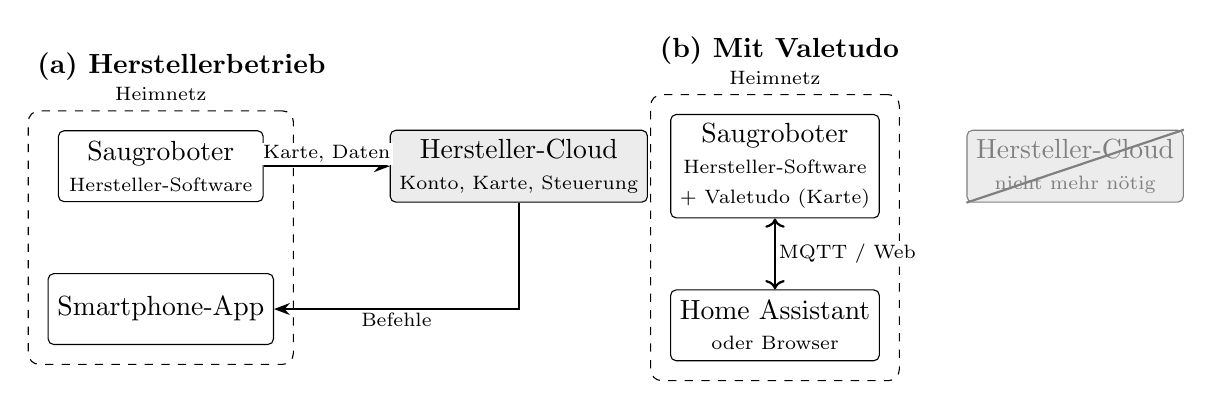
\begin{tikzpicture}[
  box/.style={draw,rounded corners=2pt,align=center,minimum width=2.6cm,minimum height=0.9cm,fill=white},
  zone/.style={draw,dashed,rounded corners=4pt,inner sep=7pt},
  arr/.style={-{Stealth[length=2mm]},thick},
  lab/.style={font=\scriptsize,fill=white,inner sep=1pt}]
% ---------- (a) Herstellerbetrieb ----------
\node[box] (r1) {Saugroboter\\[-1pt]\scriptsize Hersteller-Software};
\node[box,below=0.9cm of r1] (p1) {Smartphone-App};
\node[box,right=1.6cm of r1,fill=gray!15] (c1) {Hersteller-Cloud\\[-1pt]\scriptsize Konto, Karte, Steuerung};
\node[zone,fit=(r1)(p1),label={[font=\scriptsize]above:Heimnetz}] (z1) {};
\draw[arr] (r1) -- node[lab,above]{Karte, Daten} (c1);
\draw[arr] (c1.south) |- node[lab,pos=0.75,below]{Befehle} (p1.east);
\node[font=\bfseries,above=0.55cm of z1.north west,anchor=west] {(a) Herstellerbetrieb};
% ---------- (b) mit Valetudo ----------
\begin{scope}[xshift=7.8cm]
\node[box,minimum height=1.25cm] (r2) {Saugroboter\\[-1pt]\scriptsize Hersteller-Software\\[-1pt]\scriptsize + Valetudo (Karte)};
\node[box,below=0.9cm of r2] (h2) {Home Assistant\\[-1pt]\scriptsize oder Browser};
\node[box,right=1.1cm of r2,fill=gray!15,text=gray,draw=gray] (c2) {Hersteller-Cloud\\[-1pt]\scriptsize nicht mehr nötig};
\draw[gray,thick] (c2.south west) -- (c2.north east);
\node[zone,fit=(r2)(h2),label={[font=\scriptsize]above:Heimnetz}] (z2) {};
\draw[arr,<->] (r2) -- node[lab,right]{MQTT / Web} (h2);
\node[font=\bfseries,above=0.55cm of z2.north west,anchor=west] {(b) Mit Valetudo};
\end{scope}
\end{tikzpicture}
\end{document}
